\documentclass[../p051main.tex]{subfiles}
\graphicspath{{\subfix{../figures/}}}

\begin{document}

\chapter{Electrostatics}
\section{The Electrostatic Force}
In mechanics, all of the quantities we worked with could be described using some combination of mass, length, and time.
Starting now, though, we'll discuss a new kind of unit: charge, whose SI unit is the Coulomb (C).
It is conserved in closed systems, relativistically invariant, and quantized.
(The quantum is the charge $q_e$ carried by a proton or electron, often called the elementary charge.)

Charge can be either positive or negative, and it's well know that charges with like charges repel while those with opposite charges attract.
In particular, for two point charges $q, q_0$, the force that $q$ exerts on $q_0$ is given by
\[ \mbf{F}_E(r) = \frac{1}{4\pi \epsilon_0} \frac{qq_0}{r^2} \hat{\mbf{r}}, \]
where $\mbf{r}$ runs from $q$ to $q_0$ and $\epsilon_0$ is called the permittivity of free space.
We call this relationship the electrostatic force, also known as Coulomb's law.
Notice how it takes the exact same form as Newton's law of gravitation, simply with the added caveat that the particles may either attract or repel.

When we talk about gravity, the idea of a ``gravitational field'' often comes up to loosely describe how one massive body interacts with others around it.
We can do the same with point charges---if a charge $q$ exerts a force $\mbf{F}_E$ on $q_0$, then the electric field due to $q$ is given by
\[ \mbf{E}(r) = \frac{1}{q_0}\mbf{F}_E(r) = \frac{1}{4\pi \epsilon_0} \frac{q}{r^2} \hat{\mbf{r}}. \]
Notice how $\mbf{E}$ is independent of our choice of $q_0$, depending only on the charge $q$ and how far away it is.
Also, electric fields obey the principle of superposition---in a space with several point charges, their net electric field is found by simply summing the individual charges' fields.

\begin{example}[Electric field due to a dipole]
    Electric dipoles frequently arise in scenarios involving charged objects.
    Consider two particles with equal and opposite charges $q$ spaced a distance $d$ apart; if we look at a point a distance $x$ from the charges' midpoint, then by superposition we have
    \[ E_\textrm{dip} = 2 \cdot \frac{1}{4\pi \epsilon_0} \frac{q}{\mathcal{R}^2} \sin\theta, \]
    where $\mathcal{R}$ is the distance from $x$ to either of the charges and $\theta$ is the angle that the $x$-charge vector makes with the vertical.
    By geometry this gives
    \[ \mbf{E}_\textrm{dip} = \frac{1}{4\pi\epsilon_0} \frac{qd}{(r^2 + (d / 2)^2)^{3 / 2}} (-\hat z), \]
    with $\hat z$ pointing from the charge midpoint toward $+q$.
    In general we define the dipole moment $p \equiv qd$ to describe the separation of two opposite charges.
    (Note that $\mbf{E}_\textrm{dip} \propto r^{-3}$ for $r \gg d$.)
\end{example}

\parbox{0.55\textwidth}{
    There's a nice way to visualize these fields using electric field lines.
    An example for the case of a dipole is provided at right.
    There are a few important features to note: the lines point in the direction of the electric field, never intersect, and are only drawn in the plane of the page.
    Also, the lines start and end at positive and negative charges, respectively, unless they go off to infinity.
    Finally, the strength of the field in a given region is indicated by the density of lines there.
}\parbox{0.45\textwidth}{
    \quad\;
    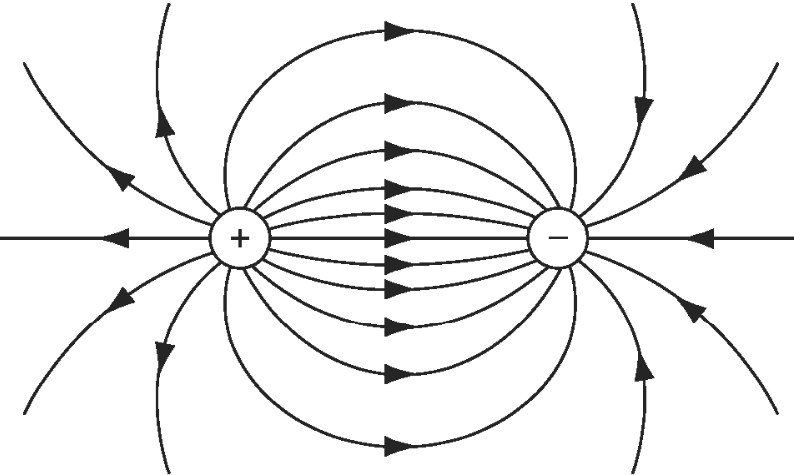
\includegraphics[width=0.4\textwidth]{electricDipole.png}
}

All of the basic principles here apply not only to collections of point charges, but also to continuous charge distributions.
In order to find the net electric field due to such a distribution, we can chop it up into a bunch of tiny pieces which can be treated as point charges.
Then by the principle of superposition,
\[ \mbf{E} = \int_V d\mbf{E} = \int_V \frac{dq}{4\pi\epsilon_0 r^2} \hat{\mbf{r}}, \]
where $V$ is the volume inhabited by the charge distribution.
Each $dq$ is a function of the charge density at that point:
\[ \text{in 1D }\; dq = \lambda \,ds, \qquad \text{in 2D }\; dq = \sigma \,dA, \qquad \text{and in 3D }\; dq = \rho \,dV, \]
where $\lambda,\sigma,\rho$ are the charge densities in their respective dimensions.
Still, in general the integral is very difficult no matter the dimension, and we usually rely on a high degree of symmetry to solve problems.
There are three main considerations here.
\begin{itemize}
    \item Different distributions lend themselves particularly well to different coordinate systems.
    For an infinite line of charge we may choose to work in cylindrical coordinates, while for a spherically symmetric distribution we may instead use spherical coordinates.

    \item For infinite charge distributions, it's useful to see if symmetry allows for the cancellation of any field components.
    In the case of an infinitely long line of charge, we'd notice that $\mbf{E}$ must only have a radial component and that, consequentially, the half-infinite lines of charge on either side of the field point have the same contribution to the net electric field.

    \item It's also useful to break up distributions in clever ways, in hopes of reducing the problem to a one-dimensional integral.
    For example, we might treat a charged sphere as a series of thin, concentric shells, each carrying a charge $\rho \,dV$, and integrate with respect to the distribution's radius.
\end{itemize}

Given how similar gravity is to the electrostatic force, it should be no surprise that Newton's shell theorem also applies to spherically symmetric charge distributions.
All of the charge ``interior'' to the field point can be treated as one big point charge, while all of that ``exterior'' to the field point cancels and can thus be ignored.

\section{Gauss's Law}
Calculating the electric field via direct integration can be quite clunky.
Fortunately, one of the fundamental equations of electromagnetism provides a much cleaner alternative.
Gauss's law states that the electric flux through a closed surface $S$ is proportional to the charge enclosed by the surface.
Symbolically,
\[ \oiint_S \mbf{E} \cdot d\mbf{A} = \frac{q_\textrm{enc}}{\epsilon_0}, \]
where $d\mbf{A}$ is an area element pointing along the outward normal and $q_\textrm{enc}$ is the net charge enclosed by $S$.
Although this statement technically holds true for any charge distribution, it's really only practical in a select few kinds of scenarios.
The idea is to construct a fictitious ``Gaussian surface'' that respects the symmetry of the electric field: for planar symmetry we may use a Gaussian box, for cylindrical symmetry a Gaussian cylinder, and for spherical symmetry a Gaussian sphere.

\begin{example}[Electric field due to a plane of charge]
    Consider an infinite plane of charge with charge density $\sigma$.
    The corresponding electric field exhibits planar symmetry---all field lines point in the $\hat z$ (upward) direction, and the magnitude depends only on $z$---so upon an arbitrary region of the plane we construct a Gaussian box with some side length $s$.

    To evaluate the surface integral, we take advantage of the fact that $\mbf{E} = E \,\hat z$ is orthogonal to the ``caps'' of the box and parallel to the lateral faces:
    \[ \oiint_\textrm{box} \hspace{-5pt} \mbf{E} \cdot d\mbf{A} = \iint_\textrm{caps} \hspace{-8pt} \mbf{E} \cdot d\mbf{A} + \cancel{\iint_\textrm{lats} \hspace{-6pt} \mbf{E} \cdot d\mbf{A}} = 2\iint_\textrm{top} \hspace{-7pt} E(|z|) \,\hat z \cdot dA \,\hat z = 2 E(|z|) \iint_\textrm{top} \hspace{-7pt} dA, \]
    so the integral evaluates to $E(|z|) \cdot 2s^2$. Since the box encloses a charge $q_\textrm{enc} = \sigma s^2$, by Gauss's law we have $E(|z|) \cdot 2s^2 = \sigma s^2$ and thus $\mbf{E}(|z|) = (\sigma / 2\epsilon_0) (\pm \hat z)$, taking $+\hat z$ for positive $z$.
\end{example}

The integral form of Gauss's law states that electric flux is proportional to enclosed charge.
This is useful, but there's another, more compact differential formulation.
First note that, by the divergence theorem, we have
\[ \iiint_V (\nabla \cdot \mbf{E}) \,dV = \oiint_{\partial V} \mbf{E} \cdot d\mbf{A} \]
for an arbitrary volume $V$ and its boundary $\partial V$.
By the integral form of Gauss's law the right-hand side turns into $q_\textrm{enc} / \epsilon_0$ or, alternatively,
\[ \iiint_V (\nabla \cdot \mbf{E}) \,dV = \iiint_V \frac{\rho}{\epsilon_0} dV. \]
Since this equivalence is true for any volume we could think of, these integrands must be equal and we get
\[ \nabla \cdot \mbf{E} = \frac{\rho}{\epsilon_0}, \]
the differential form of Gauss's law.
The ``flux density'' at a point is proportional to the charge density there.

\section{Electrostatic Potential}
Having discussed forces and fields, the next step we'll take in building a theory of electricity is to see how energy fits in.
To exploit our understanding of the electrostatic force, we'll begin by computing the amount of work $\mbf{F}_E$ does in moving a charge through an electric field.
In particular, if $q_0$ is moved between points $a$ and $b$ while in the presence of another charge $q$, then in a spherical coordinate system centered at $q$ we have
\[ W_E = \int_a^b \mathbf{F}_E \cdot d\mathbf{s} = \int_a^b \frac{q_0q}{4\pi\varepsilon_0r^2} \hat{r} \cdot (dr \,\hat{r} + r\,d\theta \,\hat{\theta} + r\sin \theta \,d\phi \,\hat{\phi}) = -\left( \frac{q_0q}{4\pi\varepsilon_0b} - \frac{q_0q}{4\pi\varepsilon_0a} \right). \]
The electrostatic force is, like gravity, a conservative force and thus has an associated potential energy related to its work by $W_E = -\Delta U_E$.
If we define $U_E(\infty) = 0$ like we often do for gravity we get
\[ U_E(r) = \frac{q_0q}{4\pi \epsilon_0 r}. \]
We might interpret this as the amount of work that must be done against $\mbf{F}_E$ in order to bring $q$ and $q_0$ into close proximity from infinite separation.
Generalizing a bit, the total potential energy in a larger system of charges is the work required to construct the system by bringing each charge in from infinite separation, one by one.
In a sense, the work is ``stored'' in the interactions between pairs of charges, and these interaction energies may be summed to determine the system's total electrostatic potential energy.

What we've essentially done here is turn a vector problem into a scalar one.
Since $\mbf{F}_E = -\nabla U_E$, in order to study the behavior of a particle under the influence of a net electrostatic force, we can simply look at the corresponding potential energy function and draw conclusions from there.
This is often much more convenient than having to deal with vectors, and in fact we can do something similar with electric fields.

If an electric field represents an electric force per unit charge, then we can define a new quantity $V$, simply called potential (measured in volts V), to represent an electric potential energy per unit charge.
Again assuming an infinite reference point, this means
\[ V(r) = \frac{U_E(r)}{q_0} = \frac{q}{4\pi \epsilon_0 r}, \]
for a point charge.
Like all of the other quantities we've discussed so far, electrostatic potential obeys the principle of superposition.
To find the potential due to a continuous distribution of charge we might again break the distribution of little chunks, approximate them as point charges, and integrate their individual contributions to the potential.

This also provides a new way to visualize electric fields.
In two dimensions we might draw equipotential lines, along which the electrostatic potential is constant.
The electric field, the negative gradient of this potential field, points normal to these lines in the direction of steepest descent.

Now, the difference in potential between two points $a$ and $b$ is unsurprisingly given by
\[ -\Delta V = \int_a^b \mbf{E} \cdot d\mbf{s}, \]
meaning we have the relationship $\mbf{E} = -\nabla V$.
Thus $\mbf{E}$ is a conservative vector field and
\[ \oint_C \mbf{E} \cdot d\mbf{s} = 0 \]
for any closed $C$.
This is a simplified version of Faraday's law (which we'll discuss in more detail later), and in differential form we can write $\nabla \times \mbf{E} = \mbf{0}$.

As a mathematical side note, we can also write $-\nabla \cdot (\nabla V) = \rho / \epsilon_0$.
This is often expressed as
\[ \nabla^2 V = -\rho / \epsilon_0 \]
where $\nabla^2$ is called the Laplacian operator, simply the sum of the second partial derivatives of $V$.
We might loosely interpret this as the ``net concavity'' of $V$ at a point---$\nabla^2 V$ is positive at points that are generally concave up, and negative at ones that are generally concave down.
Since in free space we have $\nabla^2 V = 0$, $V$ cannot have any extrema there.
It also happens that, under any physically allowed boundary conditions, solutions to this equation are unique.

\section{Conductors and Dielectrics}
Now we'll take a look at how electric fields interact with two different kinds of matter: conductors and dielectrics.
We'll begin with the simpler case of a conductor, which is a material in which each atom has at least one electron that's free to roam about.
Arguably the most important feature of such a material is that its interior has no net electric field---if a conductor is placed into an external field $\mbf{E}_0$, then its positive and negative charges will move around and create their own field $\mbf{E}_\textrm{ind}$ in the opposite direction of $\mbf{E}_0$.
Eventually there will be an equilibrium in which $\mbf{E}_\textrm{ind} = \mbf{E}_0$.

There's a few other characteristics of conductors which often come in handy.
\begin{itemize}
    \item If there is a cavity inside of a conductor, then it has no electric field.
    (Other there would be a $C$ such that $\oint_C \mbf{E} \cdot d\mbf{s} \neq 0$.)
    Charge distributes itself over the cavity's surface to make this happen.

    \item Since there is no electric field in the interior of a conductor, by Gauss's law there is no net charge anywhere inside.
    Everything is distributed over the surface.

    \item The lack of electric field also means that all points inside of a conductor are at the same potential.
    To ``ground'' a conductor (i.e., set $V = 0$) we could connect it to a huge, faraway object, like the interior of the Earth.

    \item The electric field just outside of the conductor is orthogonal to the surface.
    Any tangential component would redistribute charge so as to cancel it out.
\end{itemize}

In other materials like dielectrics, electrons are generally bound to their molecules.
However, under the influence of an external electric field, positive and negative charges can still be slightly displaced from one another.
The precise mechanism by which this occurs depends on the kind of dielectric we're talking about: polar dielectrics have a bunch of permanent dipole moments that become aligned when influenced by an electric field, while nonpolar dielectrics have no such moments until being influenced.
(In the latter case, electrons are simply displaced slightly from their normal position.)

Just like with conductors, the above rearrangement of charge induces an electric field that opposes the external field.
In the case of linear dielectrics, the magnitude of this induced field $\mbf{E}_\textrm{ind}$ is proportional to that of the applied field $\mbf{E}_0$; for such materials we can define a dielectric constant
\[ \kappa_E = \frac{E_0}{E} = \frac{E_0}{E_0 - E_\textrm{ind}}, \]
which is roughly a measure of how conductive a material is.
A perfect conductor would have $\kappa_E = \infty$.
We can also see that electric fields inside of dielectrics are diminished by a factor of $1 / \kappa$, which lines up with our intuition about conducting materials.

\section{Capacitors}
To cap off our discussion of electrostatics, we'll introduce a quantity that is fundamental to a variety of practical applications: capacitance.
Suppose we have an isolated conductor with charge $Q$ and a potential $V_0$; then the capacitance $C$ of the conductor, measured in farads (F), is the proportionality constant relating these quantities via $Q = CV_0$.
More relevant to our purposes, however, is a definition for systems of two conductors with opposite charges $\pm Q$.
Here we have $Q = C \Delta V$, where $\Delta V$ is the potential difference between the conductors.
In either case, $C$ represents the amount of charge that a system can carry per volt.

We'll focus on a special kind of capacitor comprised of two parallel plates, separated by a distance $D$, with equal and opposite charges $\pm Q$ distributed over an area $A$.
For sufficiently large plates, we can exploit our Gauss's law result from earlier---we find that the plates' individual electric fields completely cancel outside of the capacitor and add to
\[ E_{||} = \frac{\sigma}{\epsilon_0} = \frac{Q}{\epsilon_0 A} \]
on the inside.
This turns out to be a great approximation for points that are not near the capacitor's fringe.
Now, to find the capacitance of this arrangement we must first compute the potential difference between the two plates:
\[ \Delta V = \left| \int_\textrm{pos.}^\textrm{neg.} \mbf{E}_{||} \cdot d\mbf{s} \right| = \left| \int_\textrm{pos.}^\textrm{neg.} E_{||} \,ds \right| = \frac{Q}{\epsilon_0 A}D. \]
This conveniently gives us a linear relationship between $Q$ and $\Delta V$, so we immediately get
\[ Q = \left( \frac{\epsilon_0 A}{D} \right) \Delta V \;\implies\; C_{||} = \frac{\epsilon_0 A}{D}, \]
a result which should make geometric sense in the limits for $A$ and $D$.

Finally, we'll take a look at how much energy is stored in this parallel-plate capacitor.
We could compute this directly using $\Delta U = Q \Delta V$, but we'll take a more enlightening approach.
Suppose the plates are initially neutral; we can charge the capacitor by moving charges between the plates, one at a time, in total doing some amount of work
\[ W = \int_0^Q (\Delta v) \,dq = \int_0^Q \left( \frac{q}{C} \right) dq = \frac{Q^2}{2C}. \]
Since the electric field is conservative we have $W = \Delta U$, meaning this is the total amount of energy stored in the capacitor!
Some useful equivalent expressions are
\[ U = \frac{Q^2}{2C} = \frac{C (\Delta V)^2}{2} = \frac{Q \Delta V}{2}. \]
We can go a step further.
If we substitute $C = \epsilon_0 A / D$ and $\Delta V = E_{||}D$ into the latter expression, we get $U = (\epsilon_0 E_{||}^2 Ad) / 2$.
But $Ad$ is simply the volume in which the electric field exists between the plates!
So we can define a new quantity
\[ u_E = \frac{U}{\textrm{vol.}} = \frac{1}{2} \epsilon_0 E^2, \]
called the ``energy density'' of an electric field.
This suggests that we might think of the capacitor's energy as actually being stored in the field itself!

So we now have two ways of qualifying the energy stored in an electric field:
\begin{itemize}
    \item the configuration energy, which describes the work done in building the electric field, and
    \item the energy density, which describes the amount of energy stored in the field per unit volume.
\end{itemize}
This also provides us with two ways to compute the energy stored in the electric field due to some charge distribution.
We may assemble the configuration charge-by-charge, or we may simply integrate the energy density over all space.

\end{document}